\section{Method}    \label{sec:03:method}
\subsection{System overview}


Our system consists of a Finite State Machine and a (Static) Random Access Memory, as can be seen in \autoref{fig:03:system_diagram}. The FSM serves as a control unit to make sure all operations on the RAM are performed in a stable manner. The FSM is connected to a clock signal, but the RAM is not.

\begin{figure}[H]
    \centering
    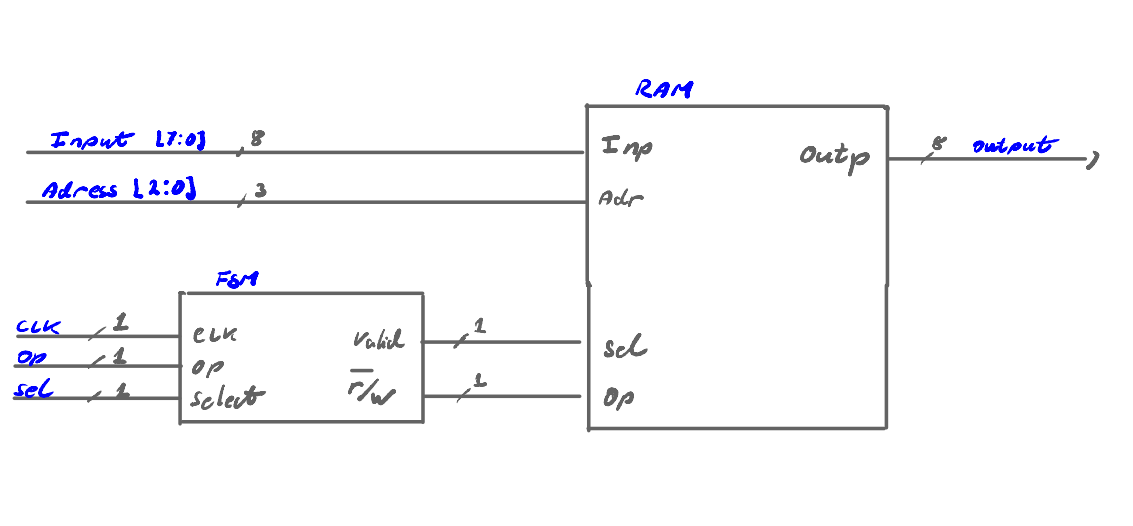
\includegraphics[width=0.8\linewidth]{LaTeX_2/Figures/memory_block_schematic.png}
    \caption{Block diagram of the system}
    \label{fig:03:system_diagram}
\end{figure}

%%%%%%%%%%%%%%%%%%%%%%%%%%%%%%%%%%%%%%%%%%%%%%%%%%%%%%%%%%%%%%%%%%%%%%%%%%%%%%%%%%%%%%%%%%%%%
%                                         RAM                                               %
%%%%%%%%%%%%%%%%%%%%%%%%%%%%%%%%%%%%%%%%%%%%%%%%%%%%%%%%%%%%%%%%%%%%%%%%%%%%%%%%%%%%%%%%%%%%%
\subsection{RAM}
The RAM subsystem consists of eight bitcells forming eight bytecells that form the full memory. It has these inputs and outputs:
\begin{itemize}
    \item \makebox[2cm]{\textit{adr} \hfill} - 3-bit address signal
    \item \makebox[2cm]{\textit{inp} \hfill} - 8-bit input data to be stored in address
    \item \makebox[2cm]{\textit{outp} \hfill} - 8-bit output data to be read from address
    \item \makebox[2cm]{\textit{op} \hfill} - either 0 for read or 1 for write
    \item \makebox[2cm]{\textit{sel} \hfill} - must be 1 for \textit{op} to affect the circuit
\end{itemize}

When the circuit is reading, meaning \textit{op} is low, the output is what is stored in the currently addressed bytecell. When it is writing, the \textit{outp} is $Z$ (high impediance), meaning it can be easily overwritten, and should not be trusted if the circuit is not in read mode with \textit{sel} high. The RAM's circuit is implemented as can be observed in \autoref{fig:03:RAM_schematic}. It consists of eight bytecell modules. The entire output bus is connected to all the bytecells in parallel, making it possible to only read from one of the bytecells at a time.

\begin{figure}[H]
    \centering
    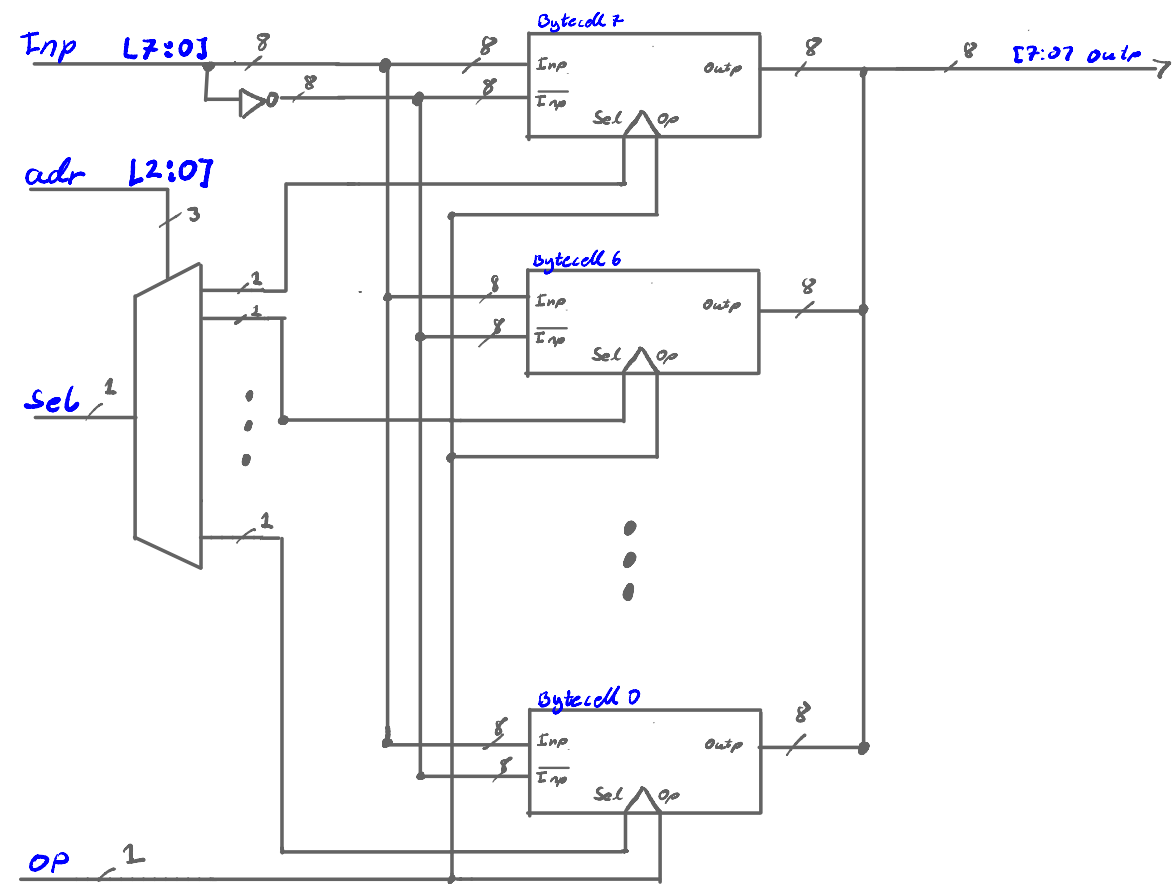
\includegraphics[width=0.8\linewidth]{LaTeX_2/Figures/ram_schematic.png}
    \caption{Schematic for the RAM subsystem}
    \label{fig:03:RAM_schematic}
\end{figure}


%%%%%%%%%%%%%%%%%%%%%%%%%%%%%%%%%%%%%%%%%%%%%%%%%%%%%%%%%%%%%%%%%%%%%%%%%%%%%%%%%%%%%%%%%%%%%
%                                         BITCELL                                           %
%%%%%%%%%%%%%%%%%%%%%%%%%%%%%%%%%%%%%%%%%%%%%%%%%%%%%%%%%%%%%%%%%%%%%%%%%%%%%%%%%%%%%%%%%%%%%
\subsubsection{The bitcell}
The bitcell concists of a D-latch and a tri-state-buffer. The logic schematic of the D-latch, connected to the transistor schematic of a tri-state-buffer, can be seen in \autoref{fig:03:bitcell_schematic}.

\begin{figure}[H]
    \centering
    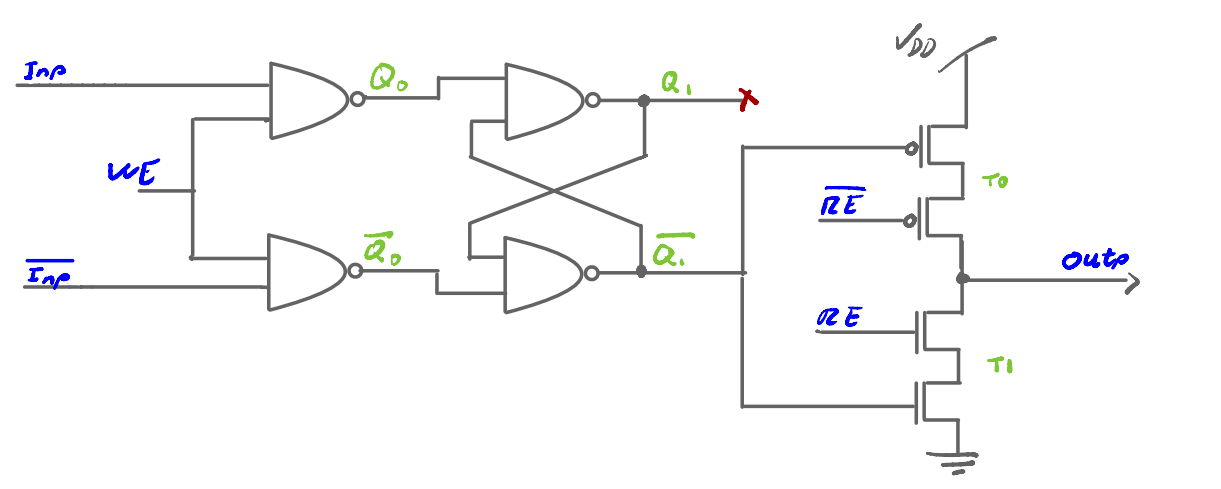
\includegraphics[width=0.8\linewidth]{LaTeX_2/Figures/bitcell_schematic.png}
    \caption{Wiring schematic for the bitcell module}
    \label{fig:03:bitcell_schematic}
\end{figure}

The bitcell has inputs and outputs:
\begin{itemize}
    \item \makebox[2cm]{\textit{inp} \hfill} - The input bit to be stored
    \item \makebox[2cm]{\textit{inpn} \hfill} - (input not) The inverse of the input bit
    \item \makebox[2cm]{\textit{outp} \hfill} - The output when the circuit is read
    \item \makebox[2cm]{\textit{WE \hfill}} - Write Enable, must be high to store a new value
    \item \makebox[2cm]{\textit{RE \hfill}} - Read Enable, must be high to set outp to the stored value
    \item \makebox[2cm]{\textit{REN} \hfill} - (Read Enable Not) inverted of \textit{RE}
\end{itemize}

The inverse stored value sits in the node $\overline{Q_1}$. We choose to implement the bitcell with a tri-state-buffer in order to make the output high impedance ($Z$) when \textit{RE} is low. This is to ensure that the shared output bus in the RAM module can be overwritten by the selected bytecell module if \textit{RE} is high. This simplifies the rest of the design, since there is no need for a multiplexer to choose which address to read data from.

\subsubsection{Bitcell leakage}
The leakage current of each bitcell is a sum of the leakage current of all its transistors. In total there are 20 transistors in each bitcell, 10 NMOS and 10 PMOS. The leakage current of one NMOS can be estimated from equation \ref{eq:02:drain_current}. To reduce the leakage current, the right side of this equation can be reduced by tuning the width-to-length ratio. Hence, our choice of transistor sizes, as shown in table \ref{tab:03:transistor_size}, are chosen to reduce this ratio (within the allowed specifications of the assignment).

\begin{table}[H]
    \centering
    \caption{Chosen size of P- \& N-MOS transistor.}
    \label{tab:03:transistor_size}
    \begin{tabular}{|c|c|}
                                \hline
         W  &  \SI{101}{nm} \\  \hline
         L  &  \SI{299}{nm} \\  \hline
    \end{tabular}
\end{table}

In the next section the slow-slow (SS) corner has the slowest operation time of all the simulation corners as seen in \autoref{fig:04:write}. The voltage supply was chosen to be $V_{DD} = \SI{0.99}{V}$ based on early simulations. This value provided us with the most stable and functional bitcell for all of the operational corners within the task's read/write requirements of \SI{3}{ns} as can be seen in \autoref{fig:03:write_times}.

\begin{figure}[H]%
\centering
\subfigure[$V{dd} = \SI{0.6}{V}$]{%
\label{fig:first}%
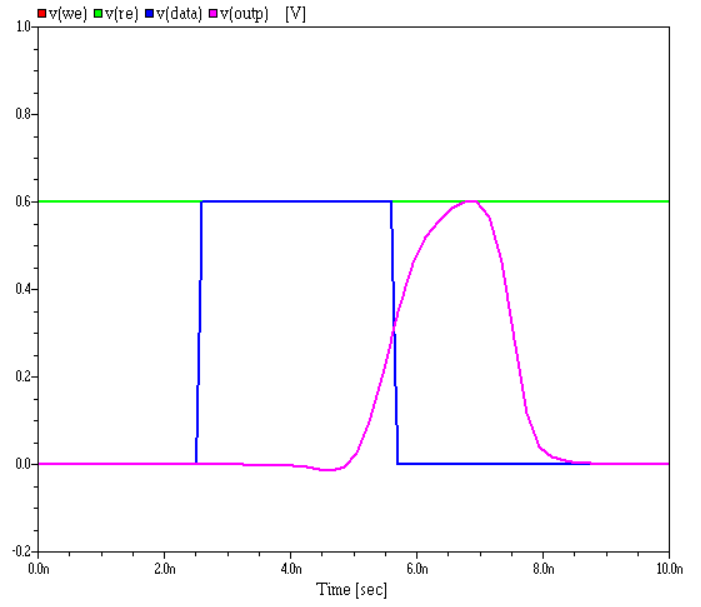
\includegraphics[height=1.5in]{LaTeX_2/Figures/write060V.png}}%
\qquad
\subfigure[$V{dd} = \SI{0.8}{V}$]{%
\label{fig:second}%
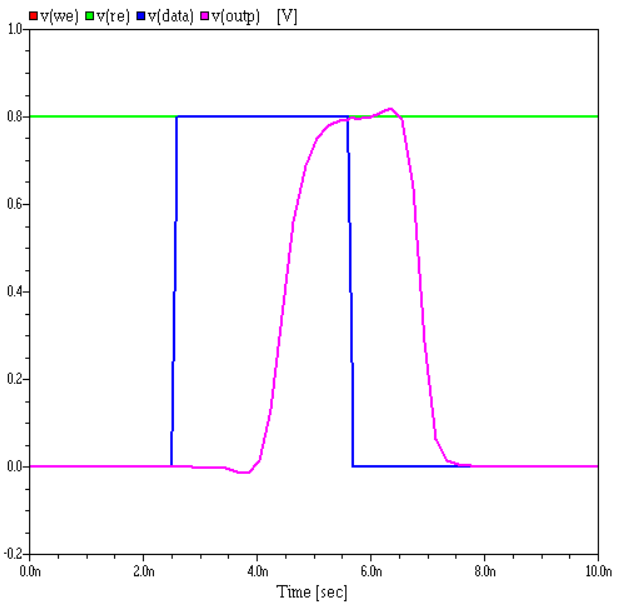
\includegraphics[height=1.5in]{LaTeX_2/Figures/write080V.png}}%
\qquad
\subfigure[$V{dd} = \SI{0.99}{V}$]{%
\label{fig:third}%
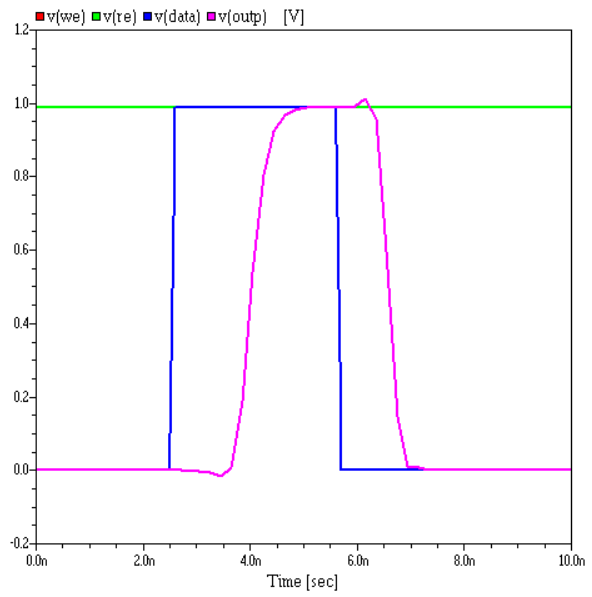
\includegraphics[height=1.5in]{aimSpice/plots/plotsSS/write.png}}%
\caption{Write times for the \textit{SS} corner at different supply voltages, $V_{dd}$. The input pulse is exactly \SI{3}{ns} long.}
\label{fig:03:write_times}
\end{figure}

%%%%%%%%%%%%%%%%%%%%%%%%%%%%%%%%%%%%%%%%%%%%%%%%%%%%%%%%%%%%%%%%%%%%%%%%%%%%%%%%%%%%%%%%%%%%%
%                                         BYTECELL                                          %
%%%%%%%%%%%%%%%%%%%%%%%%%%%%%%%%%%%%%%%%%%%%%%%%%%%%%%%%%%%%%%%%%%%%%%%%%%%%%%%%%%%%%%%%%%%%%
\subsubsection{The bytecell}
The bytecell consists of 8 bitcells and an F-block (function block) meant to translate the input signals of the bytecell to the required inputs of each of its bitcells. The bitcells all write their outputs to 8 different wires, which we refer to as the databus. The bytecell schematic can be seen in \autoref{fig:03:bytecell_schematic}.

\begin{figure}[H]
    \centering
    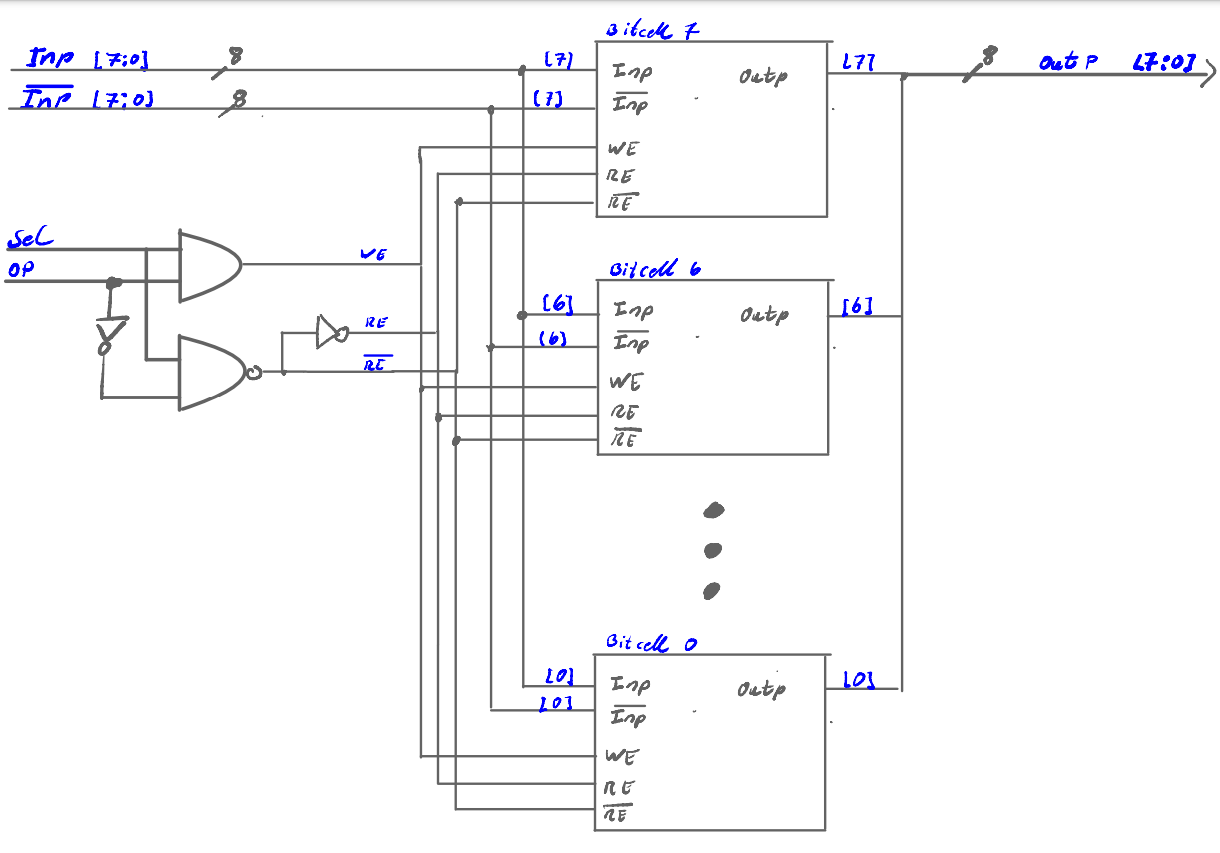
\includegraphics[trim=0cm 0cm 0cm 0.3cm, clip, width=0.8\linewidth]{LaTeX_2/Figures/bytecell_schematic.png}
    \caption{Wiring schematic for the bytecell module}
    \label{fig:03:bytecell_schematic}
\end{figure}

The inputs and outputs of the bytecell are almost identical to those of the RAM, with the exception of there being no address signal, and the input having to be written both normally and inverted. Having the inverse signal bus at this level means saving transistors, as there will be one inverter for all of the 8 databus wires one level higher, instead of one inverter for every bitcell. The downside to this solution is that we need more wires connecting each module, which in turn can create more noise and disruptions internally. If the inverted wires are printed as differential pairs, the noise issue will be minimized. 

The control logic on the left was designed to set \textit{WE} high only when \textit{op} and \textit{sel} are high, and to set \textit{RE} high only when \textit{op} is low and \textit{sel} is high. Otherwise, both \textit{WE} and \textit{RE} are set to low. The truth table can be seen in \autoref{tab:03:F-block}.

\begin{table}[H]
    \centering
    \caption{The truth table for the control logic in \autoref{fig:03:bytecell_schematic}.}
    \begin{tabular}{|c|c||c|c|}
        \hline
        \textit{op}  & s\textit{sel} & \textit{WE} & \textit{RE} \\ \hline
        0   & 0   &   0         & 0           \\
        0   & 1   &   0         & 1           \\
        1   & 0   &   0         & 0           \\
        1   & 1   &   1         & 0           \\ \hline
    \end{tabular}
    \label{tab:03:F-block}
\end{table}

\subsubsection{Demux}
The demultiplexer (demux) that can be seen on the left in \autoref{fig:03:RAM_schematic} sends \textit{inp} (\textit{sel} in \autoref{fig:03:RAM_schematic}) to a single addressed \textit{outp} (a bytecell), according to the address in \textit{adr}. All the other \textit{outp} are set to low, except for the one that is addressed. The demux schematic is as shown in \autoref{fig:03:demux_schematic}.

\begin{figure}[H]
    \centering
    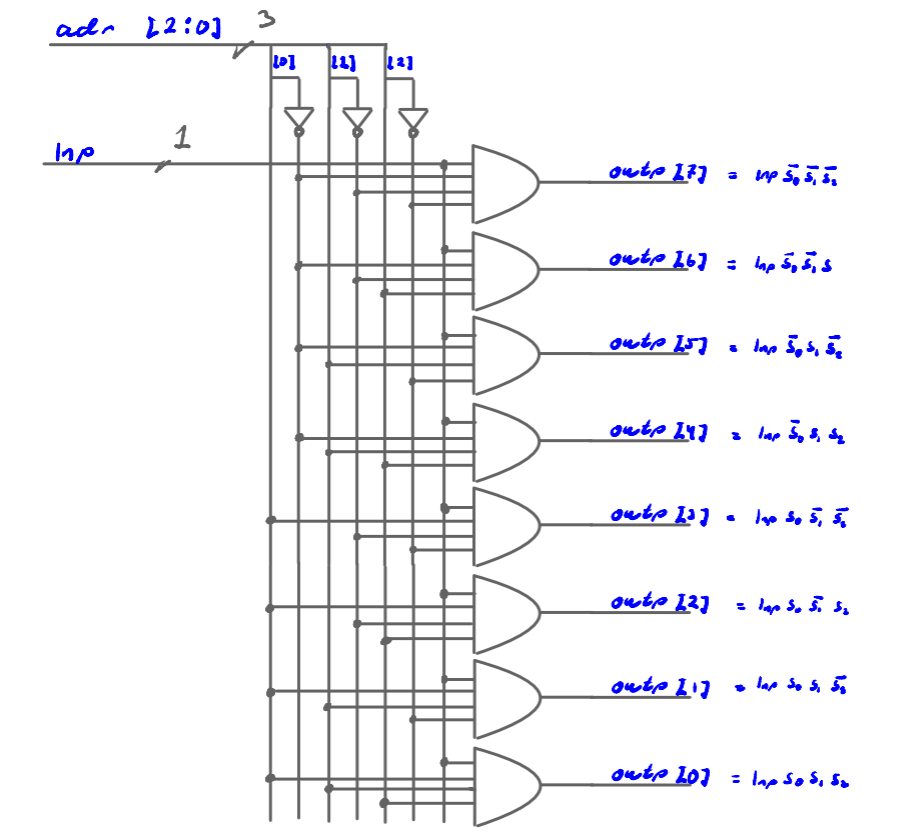
\includegraphics[width=0.75\linewidth]{LaTeX_2/Figures/demux1to8_schematic.png}
    \caption{A schematic of the demux}
    \label{fig:03:demux_schematic}
\end{figure}

%%%%%%%%%%%%%%%%%%%%%%%%%%%%%%%%%%%%%%%%%%%%%%%%%%%%%%%%%%%%%%%%%%%%%%%%%%%%%%%%%%%%%%%%%%%%%
%                                         FSM                                               %
%%%%%%%%%%%%%%%%%%%%%%%%%%%%%%%%%%%%%%%%%%%%%%%%%%%%%%%%%%%%%%%%%%%%%%%%%%%%%%%%%%%%%%%%%%%%%
\subsection{FSM}
The finite state machine is meant to work as an interface for stable and secure use of the RAM subsystem. Its design is based on what was demanded in the project description \cite{oppgavebeskrivelse}. The required design can be seen in \autoref{fig:03:state_diagram}. 

\begin{figure}[H]
    \centering
    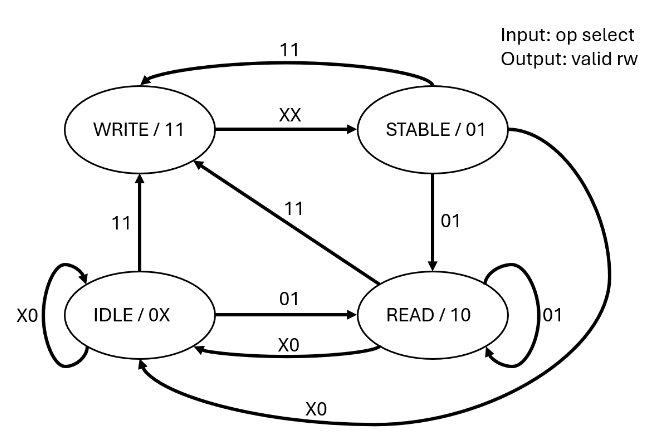
\includegraphics[width=0.6\linewidth]{LaTeX_2/Figures/state_diagram.png}
    \caption{Desired state diagram \cite{oppgavebeskrivelse}}
    \label{fig:03:state_diagram}
\end{figure}

In order to design the aforementioned system state codes were made as can be seen in \autoref{tab:03:state_code}. Then a truth table was created in order to find the logical relations between inputs and outputs in \autoref{tab:03:FSM_truth_table}, where:
\begin{itemize}
    \item A - current state of register $R0$.
    \item B - current state of register $R1$.
    \item C - input \textit{op}.
    \item D - input \textit{sel}.
    \item E - next state of register $R0$.
    \item F - next state of register $R1$.
    \item G - output \textit{valid}.
    \item H - output \textit{rw}.
\end{itemize}


\begin{table}[H]
    \caption{State codes.}
    \centering
    \begin{tabular}{|l|c|}
        \hline
        State   &   Code    \\  \hline
        IDLE    &   0 X     \\  
        STABLE  &   0 1     \\
        READ    &   1 0     \\
        WRITE   &   1 1     \\  \hline
    \end{tabular}
    \label{tab:03:state_code}
\end{table}


\begin{table}[H]
    \caption{Truth table for Finite State Machine.}
    \centering
    \begin{tabular}{|cc|cc|cc|cc|}
        \hline
        \multicolumn{2}{|c|}{State} & \multicolumn{2}{c|}{Input} & \multicolumn{2}{c|}{State nxt} & \multicolumn{2}{c|}{Output}  \\ \hline
                     &              & \textit{op} & \textit{sel} &                &               & \textit{valid} & \textit{rw} \\
        A            & B            & C           & D            & E              & F             & G     & H                    \\ \hline
        0            & 0            & 0           & 0            & 0              & X             & 0     & X                    \\
        0            & 0            & 0           & 1            & 1              & 0             & 0     & X                    \\
        0            & 0            & 1           & 0            & 0              & X             & 0     & X                    \\
        0            & 0            & 1           & 1            & 1              & 1             & 0     & X                    \\
        0            & 1            & 0           & 0            & 0              & X             & 1     & 0                    \\
        0            & 1            & 0           & 1            & 1              & 0             & 1     & 0                    \\
        0            & 1            & 1           & 0            & 0              & X             & 1     & 0                    \\
        0            & 1            & 1           & 1            & 1              & 1             & 1     & 0                    \\
        1            & 0            & 0           & 0            & 0              & X             & 0     & 1                    \\
        1            & 0            & 0           & 1            & 1              & 0             & 0     & 1                    \\
        1            & 0            & 1           & 0            & 0              & X             & 0     & 1                    \\
        1            & 0            & 1           & 1            & 1              & 1             & 0     & 1                    \\
        1            & 1            & 0           & 0            & 0              & 1             & 1     & 1                    \\
        1            & 1            & 0           & 1            & 0              & 1             & 1     & 1                    \\
        1            & 1            & 1           & 0            & 0              & 1             & 1     & 1                    \\
        1            & 1            & 1           & 1            & 0              & 1             & 1     & 1                    \\ \hline
    \end{tabular}
    \label{tab:03:FSM_truth_table}
\end{table}

Using the logical relations between the inputs, outputs, current states and next states in \autoref{eq:03:boolean_equation}, we designed an circuit implementation of the state machine in \autoref{fig:03:FSM_schematic}.

\begin{equation}
    \begin{split}
        E   &=  D \cdot \overline{A \cdot B}\\
        F   &=  A \cdot B + C \cdot D       \\
        G   &=  B                           \\
        H   &=  A
    \end{split}
    \label{eq:03:boolean_equation}
\end{equation}

\begin{figure}[H]
    \centering
    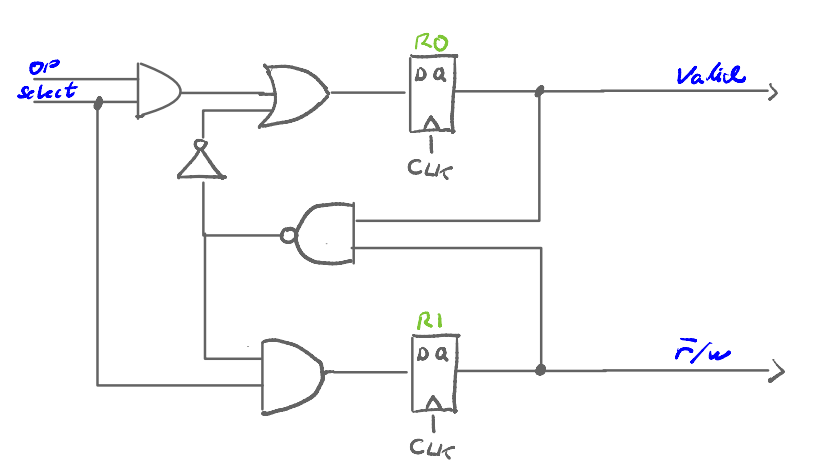
\includegraphics[width=0.8\linewidth]{LaTeX_2/Figures/fsm_schematic.png}
    \caption{Wiring schematic for the FSM logic.}
    \label{fig:03:FSM_schematic}
\end{figure}